\documentclass[spanish]{beamer}
\usepackage[spanish]{babel}
\usepackage{xifthen}

\usetheme{default}
\usecolortheme{crane}
\beamertemplatenavigationsymbolsempty
\setbeamercovered{transparent}

\newcommand{\declarefunction}[2][]{%
    \ifthenelse{\isempty{#1}}{%
        \expandafter\newcommand\csname #2\endcsname{\mathsf{#2}}%
    }{%
        \expandafter\newcommand\csname #1\endcsname{\mathsf{#2}}%
    }%
}
\declarefunction{thin}
\declarefunction{pw}

\title{Thinness y Algoritmos Parametrizados}
\author{Eric Brandwein}
\date{22 de abril de 2024}

\begin{document}

\begin{frame}
  \titlepage
\end{frame}

\section{Thinness}
\begin{frame}{Thinness}{Solución consistente}
    \begin{definition}[Solución consistente]
        Una \emph{solución consistente usando $k$ clases} para un grafo $G$ es un par $(\prec, S)$ donde 
        \begin{itemize}
            \item $\prec$ es un orden estricto total en $V(G)$, y 
            \item $S$ es una partición de $V(G)$ en $k$ clases,
        \end{itemize}
        tal que, para cada tres vértices $u\prec v \prec w$ de $G$, si
        \begin{itemize}
            \item $u$ y $v$ pertenecen a la misma clase en $S$, y
            \item $u$ y $w$ son adyacentes en $G$,
        \end{itemize}
        entonces $v$ y $w$ son adyacentes en $G$.
    \end{definition}
\end{frame}

\begin{frame}{Un ejemplito}
    \begin{center}
        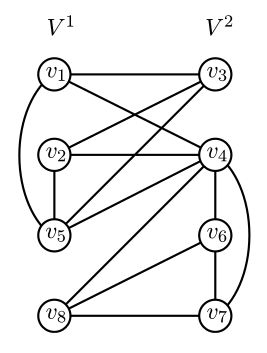
\includegraphics[width=0.5\textwidth]{img/ejemplo_thinness.png}
    \end{center}
\end{frame}

\begin{frame}{Thinness}
    \begin{definition}[$k$-thin]
        Un grafo es \emph{$k$-thin} cuando admite una solución consistente usando $k$ clases.
    \end{definition}

    \pause
    \begin{definition}[Thinness]
        La \emph{thinness} de un grafo $G$, denotada $\thin(G)$, es el mínimo entero $k$ tal que $G$ es $k$-thin.
    \end{definition}
\end{frame}

\begin{frame}{Thinness}
    \begin{block}{\textsc{Thinness}}
        \textbf{Entrada:} Un grafo $G$ y un entero $k$.

        \textbf{Salida:} ¿$\thin(G) \leq k$?
    \end{block}

    \pause
    \begin{theorem}[Y. Shitov, \cite{thinness-np-complete}]
        \textsc{Thinness} es NP-completo.
    \end{theorem}
\end{frame}

\begin{frame}{Thinness}
    ¿Quizá hay clases de grafos para las cuales \textsc{Thinness} es polinomial?
    \pause

    \begin{theorem}[Thinness de árboles, \cite{thinness-of-trees}]
        Existe un algoritmo que toma tiempo $O(n \log n)$ para \textsc{Thinness} cuando el grafo de entrada es un árbol. 
    \end{theorem}

    \pause    
    \begin{theorem}[Thinness de cografos, \cite{tesis-diego}]
        Un cografo tiene thinness mayor o igual a $t$ si y sólo si contiene a $\overline{t K_2}$ como subgrafo inducido. 
    \end{theorem}

\end{frame}

\begin{frame}{Thinness}
    ¿Hay algún parámetro de un grafo que nos permita saber cuán fácil es calcular su thinness?
    \vspace{1em}

    \pause
    Introducing... \textbf{Complejidad Parametrizada}.
\end{frame}

\begin{frame}{Problemas clásicos}
    \begin{itemize}
        \item Entrada: Cadena de bits
        \item Salida: Sí o No
        \item Complejidad temporal medida en el \textbf{tamaño de la entrada}.
    \end{itemize}
\end{frame}


\begin{frame}{Problemas parametrizados}
    \begin{itemize}
    \item Entrada: Cadena de bits \textbf{+ parámetro $k$ (un entero)}
    \item Salida: Sí o No
    \item Complejidad temporal medida en el \textbf{tamaño de la entrada y el valor de $k$}.
    \end{itemize}
\end{frame}

\begin{frame}{Clase de complejidad FPT}
    \begin{definition}[FPT]
    Un problema parametrizado está en la clase \emph{FPT (Fixed Parameter Tractable)} si existe un algoritmo que lo resuelve en tiempo $O(f(k) \cdot n^c)$, donde $f$ es una función computable y $c$ es una constante.
    \end{definition}
    \pause

    Ejemplos:
    \begin{itemize}
        \item<2-> $k$-\textsc{Vertex cover}.
        \item<3-> Muchos problemas parametrizados por el treewidth del grafo de entrada.
        \item<4-> \textsc{Thinness} parametrizado por el cluster module number, neighborhood diversity, twin-cover, o vertex cover del grafo de entrada.
    \end{itemize}
\end{frame}

\begin{frame}{Objetivos}
    \begin{itemize}[<+->]
        \item Encontrar parámetros que permitan obtener algoritmos FPT para \textsc{Thinness}.
        \item Relacionar la thinness con otros parámetros de grafos.
        \begin{itemize}
            \item Por ejemplo, antes se sabía que $\thin(G) \leq \pw(G) + 1$. Ahora se sabe que $\thin(G) \leq \pw(G)$. Gran avance para la ciencia mundial.
        \end{itemize}
        \item Decidir la complejidad de \textsc{Thinness} cuando el parámetro es el $k$ de entrada.
        \begin{itemize}
            \item Sabemos que cuando $k=1$ el problema es polinomial (los grafos de thinness 1 son exactamente los grafos de intervalos). No tenemos ni idea para $k \geq 2$.
        \end{itemize}
        \item Encontrar todo esto para parámetros relacionados: proper thinness, thinness dada partición, etc.
        \begin{itemize}
            \item Dato de color: si me das el orden de los vértices, puedo encontrar una partición óptima que sea consistente en $O(n^3)$.
        \end{itemize}
        \item etc.
    \end{itemize}
\end{frame}

\begin{frame}{Referencias}
    \bibliographystyle{plain}
    \bibliography{references}
\end{frame}


\end{document}
